\documentclass[a4paper,12pt]{article}

\usepackage[section]{placeins}

\usepackage[]{hyperref}
\usepackage{cleveref}

\usepackage[sorting=none,backend=bibtex,style=authoryear]{biblatex}
\bibliography{akb29_report}

\usepackage{float}

\usepackage{siunitx}

\usepackage{times}
\usepackage{graphicx,epsfig}
\usepackage[leftcaption]{sidecap}
\usepackage{subfigure} % figures can have sub chunks
\usepackage{geometry} % this maxes page usage, making the below unnecessary
\textwidth = 6.75in
\oddsidemargin = -0.25in
\textheight = 10in
\topmargin = -0.5in
\usepackage{fancyhdr}
\usepackage{pdfpages}

\usepackage{enumitem}
\setlist{nolistsep}

\pagestyle{fancy}
\lhead{{\it Alex Birch (with Chris Clarke)}}
\chead{Wall Following LEGO Robots}
\rhead{Coursework 1}
\lfoot{}
\cfoot{\thepage}
\rfoot{}

\newcommand{\goodgap}{%
 \hspace{\subfigtopskip}%
 \hspace{\subfigbottomskip}}

\newcommand{\citeauthoryear}[1]{%
 \citeauthor{#1}%
 ~(\citeyear{#1})}

\title{Coursework 1:  Wall Following with a LEGO Robot}
\author{Alex Birch (with partner Chris Clarke)}


\begin{document}
\maketitle

\section{Introduction}
We adopted a reactive approach to wall-following (as opposed to planning), for two reasons:
\begin{itemize}
\item The robot's movement through the world could not be reliably tracked as a plan is followed; its proprioception was limited. This concept refers to the ability for the robot to keep track of its body parts, summarised in \parencite{lee2002proprioception}.
\item \citeauthoryear{brooks1991intelligence} argues we cannot produce valid intelligence by planning actions based on a representation of the world, since no representation could wholly represent the world.
\end{itemize}
%A bump sensor was mounted far in front of the robot. Its purpose was to detect frontal collisions early enough to prevent the wheels gaining purchase on the wall. Since this distance limit was tangible, collision with the sensor would resist further movement in the same direction. 
%This was to support the position-agnostic assumptions we made. 
A subsumption architecture --- as described in \parencite{brooks1991intelligence} --- complemented our reactive approach. It allowed lower layers (such as `recover from collision') to inhibit immediate goals (such as `follow wall'). This was critical for suppressing actions that were generating inappropriate behaviour. Sensors were all running, all the time, and created the impulse for action. In this way, our action was coupled to perception; our `modules' were behaviours.

Overall the goal was to be effective at reacting. We aimed for the robot to be effective at pronating to the next wall after rounding a corner. \textbf{Our hypothesis is that `change in separation' from that wall decreases, for as long as the robot follows the new wall.} In other words: irrespective of how chaotic the robot motion is as it rounds a corner, it should converge on a consistent distance from the wall, given enough wall to follow. \textbf{Our null hypothesis is that `change in separation' from the wall is unrelated to how far the robot follows the new wall.}
\section{Approach}
My partner was Chris Clarke. I wrote the robot code and built the robot. He gave some input on these, and edited the video. We measured performance together, but analysed the dataset independently.

For collision response, we recruited a mixture of avoidance and recovery. Our robot was designed to follow walls on the left only. It was largely blind on the right-hand-side, but invested a higher resolution in the side it was aiming to follow. Its bump sensor physically guaranteed a berth from obstacles, providing intelligence through morphology \parencite{pfeifer2005morphological}.

Ultrasound sensing was known to be noisy, so we did not initiate maneuvers based on single samples; a percentage of positive readings over some timeframe was required to produce a strong enough impulse to invoke action.

The robot initiates by moving forward until the bump sensor depresses. This is considered the first wall, and the robot turns to keep it on its left, following it. `Following' takes a history of range comparisons. The robot recognises `increase over time' as divergence, and steers to correct this. This fine correction of steering was called `pronation'.

The robot had primitives for left and right facing maneuvers. A frontal collision (detected by bump sensor) would trigger the right-turn behavior. A consistent sensor reading of `distance\_max' from its left ultrasound sensor would trigger a left-turn. These did not need to be perfect \ang{90} turns, because pronation would correct the robot's angle to the wall afterward. The same mechanism also supported following non-perpendicular walls.

Behaviour inhibition was implemented by modeling maneuver primitives as queues of motor outputs, to be attended on each timestep. Sensors ran every timestep also. Thus if a bump was detected during a maneuver, the motor queue could be cleared, aborting the maneuver in favor of a newer, more appropriate action. Layering was achieved by giving each sensor a priority; for example, bumping required urgent recovery, so could interrupt any other behaviour. The overarching `wall-following' behaviour was an implicit, emergent layer that was achieved by subsuming all lower behaviours whenever sensors deemed appropriate.

Overall the robot was optimized for reacting quickly to an unpredictable environment; its architecture allowed it to interrupt maneuvers. Its three motors allowed it to make fine steering adjustments without compromising speed. Its static sensor mounting meant that sensing was immediate, and not a bottleneck on choosing action. Its pronation behaviour enabled it to maintain a predictable position.

We evaluated part of our robot's reaction effectiveness, by measuring its pronation effectiveness. Since the goal was to stay parallel to the wall, we measured its change in distance from the wall after rounding a corner. This change was measured by placing an array of rulers along a wall (at 30cm intervals), reading what distance the robot's back-left wheel was from the wall as it passed each one. As an independent variable, we varied the angle around which the robot had to turn to meet the new wall (ie, how obtuse the two walls were).

\section{Results}

%\includepdf[pages={1}]{Convergence.pdf}
%\fbox{\includegraphics[trim=0.0cm 11cm 0.0cm 11cm,clip]{Convergence.pdf}}
%\centerline{\fbox{\includegraphics[viewport=0 0 390 610,clip,width=8in]{Convergence.pdf}}}



%\includepdf[pages={1}]{Convergence2.pdf}

\Cref{fig:coursem90,fig:coursem8,fig:course0,fig:course90} show photos of each experiment.
\Cref{fig:rawm90,fig:rawm8,fig:raw0,fig:raw90} provide the raw data measured at each milestone on the wall.
\Cref{fig:derivm90,fig:derivm8,fig:deriv0,fig:deriv90} provide the distance deltas between each milestone. Shown also is a mean average of all 4 tests, as well as standard deviation and error in that sample. The graphs that follow are drawn from these data.

\Cref{fig:turnm90} shows a moderate negative correlation; each milestone along the wall, the robot becomes more parallel.
\Cref{fig:turnm8} shows a strong negative correlation; each milestone along the wall, the robot becomes more parallel.
\Cref{fig:turn0} shows a weak negative correlation; each milestone along the wall, the robot becomes more parallel. In this no-turn case, the robot does not have to converge so much as it just finished following a wall of the same angle.
\Cref{fig:turn90} shows a weak positive correlation; each milestone along the wall, the robot becomes less parallel.

\section{Discussion}

All tests save for \ang{90} show a negative correlation for distance change along the wall, meaning that the robot's distance from the wall changes less and less. These are consistent with the hypothesis. The anomalous \ang{90} results were unexpected, and in fact disagree with the hypothesis. These outliers might be attributable to the measurement approach; perhaps for right-turns we should have taken measurements from the right wheel instead, as it leads the turning. Overall there is a large amount of error; more attempts, more wall angles, and more measurement milestones would make the results more reliable.

\section{Conclusion}

In conclusion, our robot demonstrates the ability to follow parallel to (at least) convex walls. There is weak and potentially invalid support for its being unable to follow concave walls. The robot can thus react effectively to (at least) convex wall following situations.

\section{Figures}

\begin{figure}[ht]
\centerline{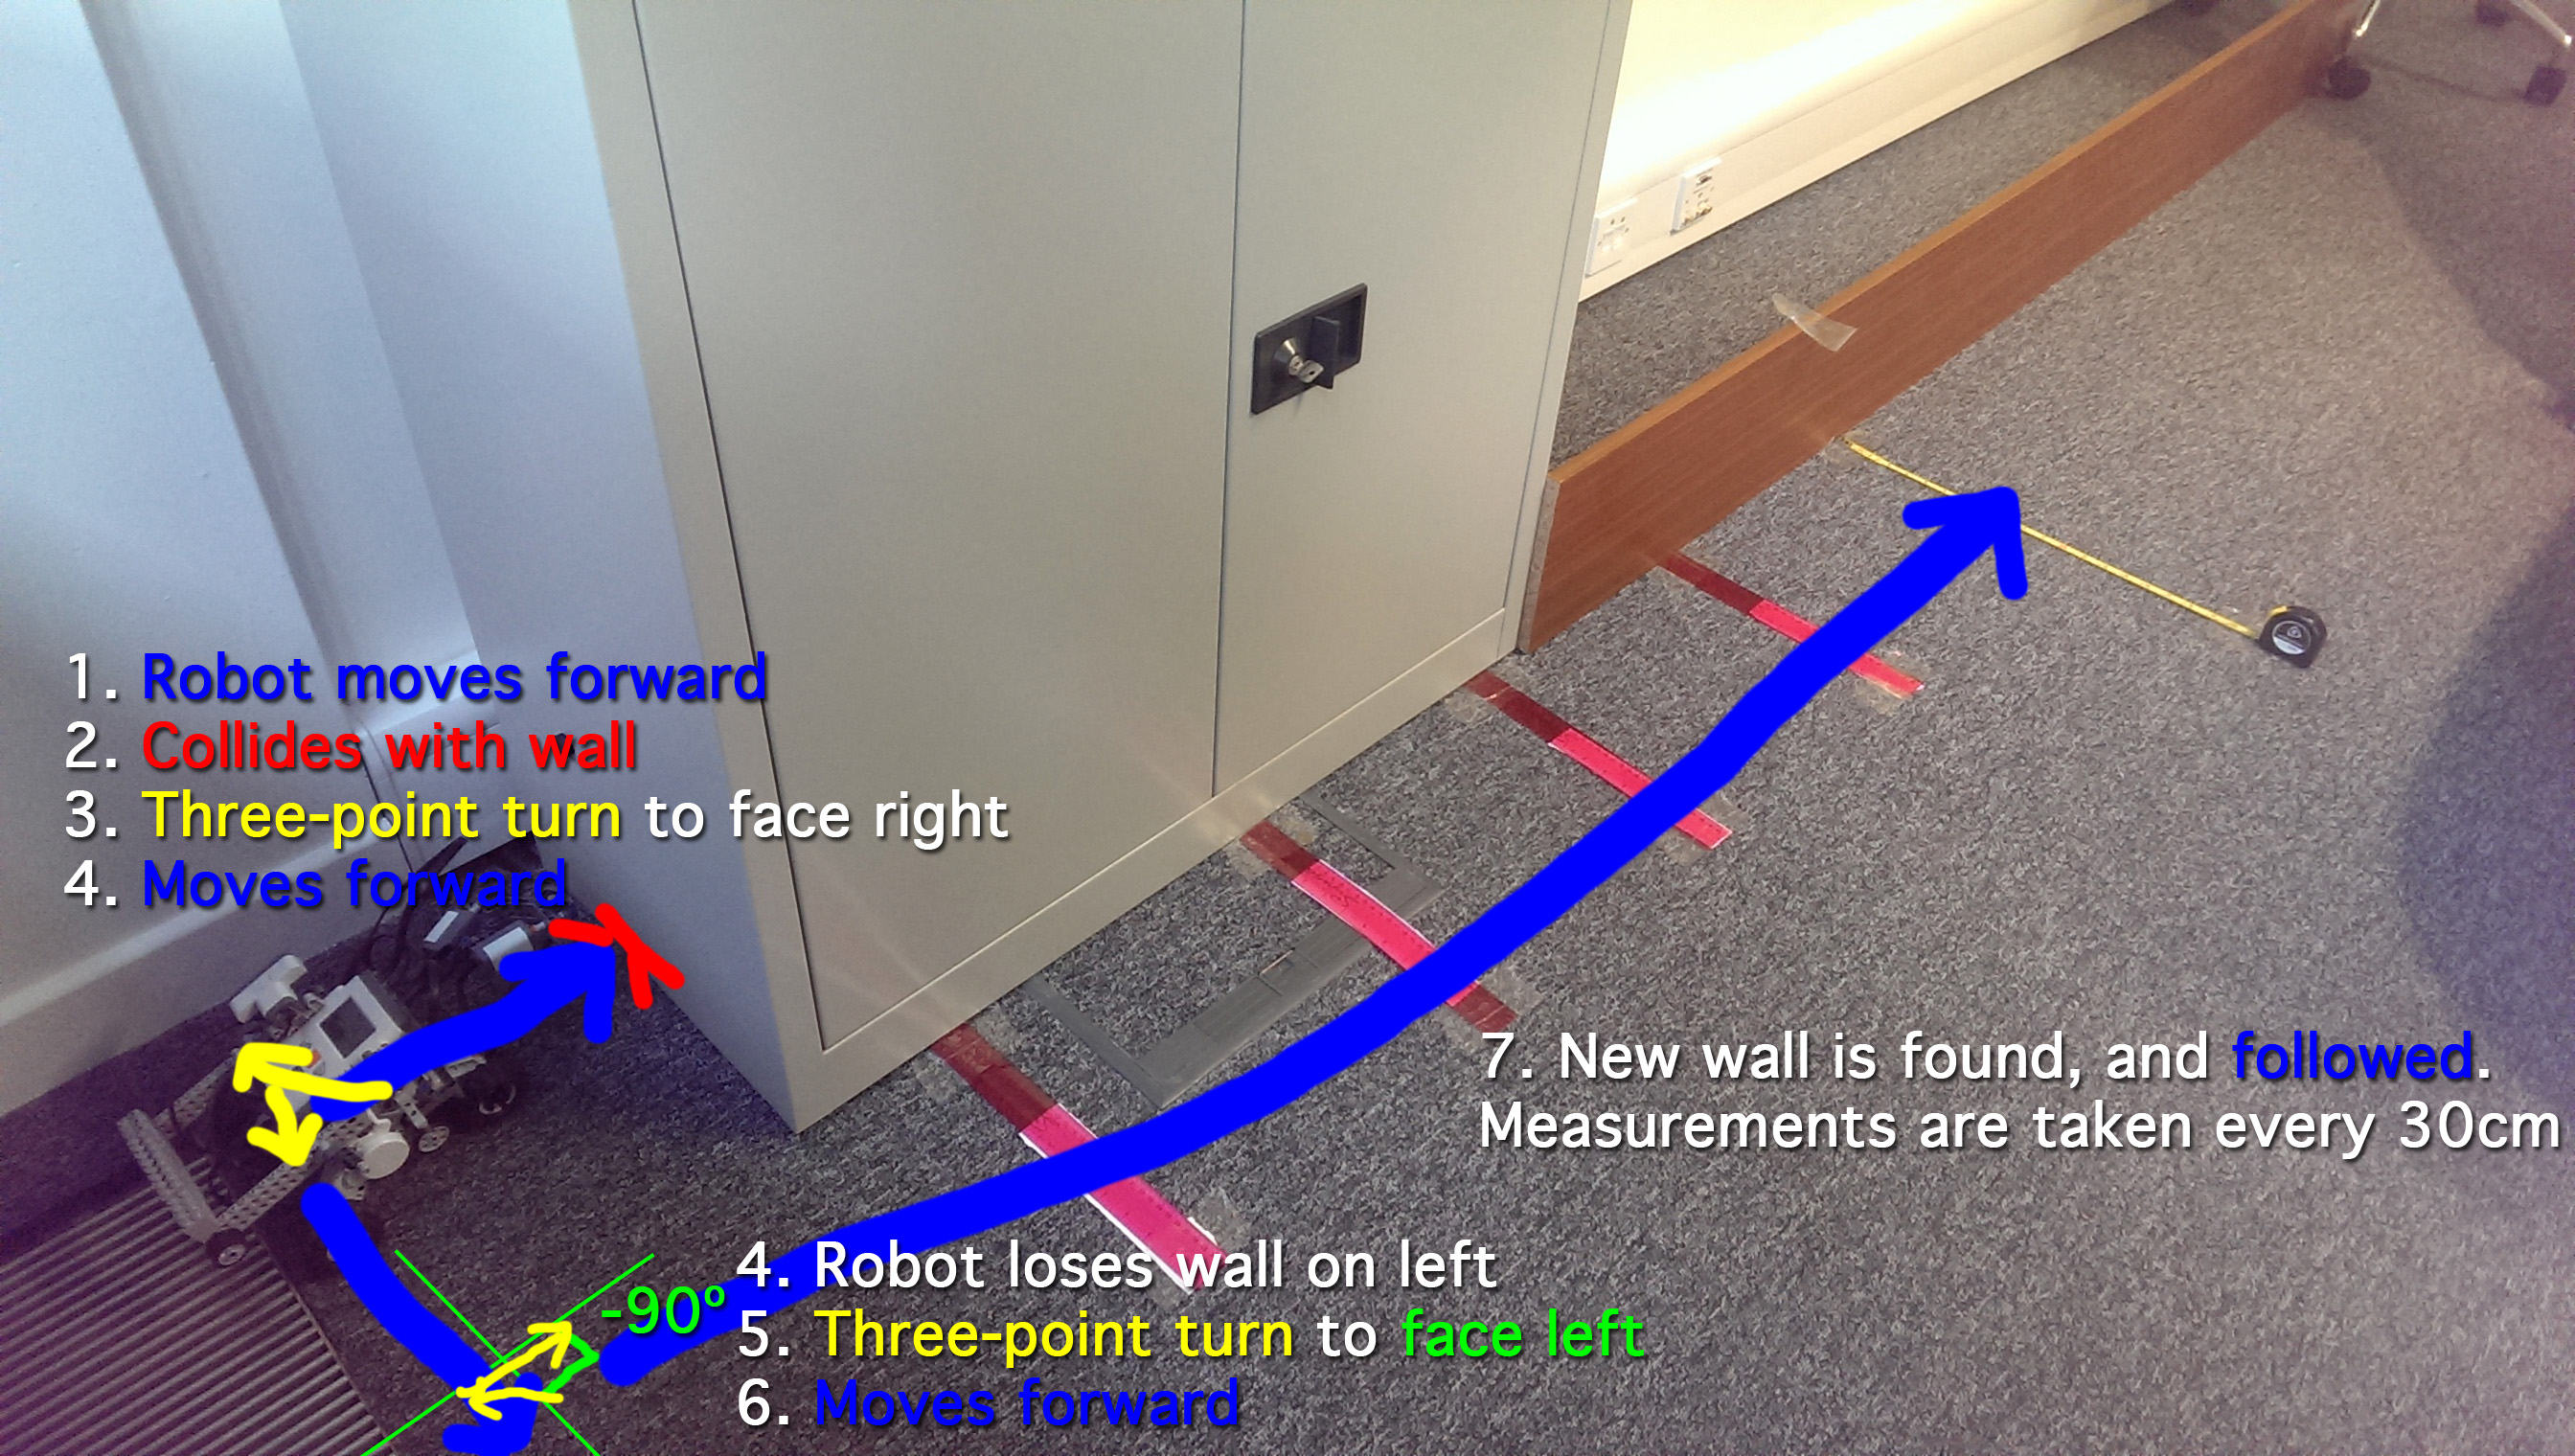
\includegraphics[width=8in]{CourseM90_Edit.jpg}}
\caption{\ang{-90} wall following (drawn path is an example for illustrative purposes)}
\label{fig:coursem90}
\end{figure}

\begin{figure}[ht]
\centerline{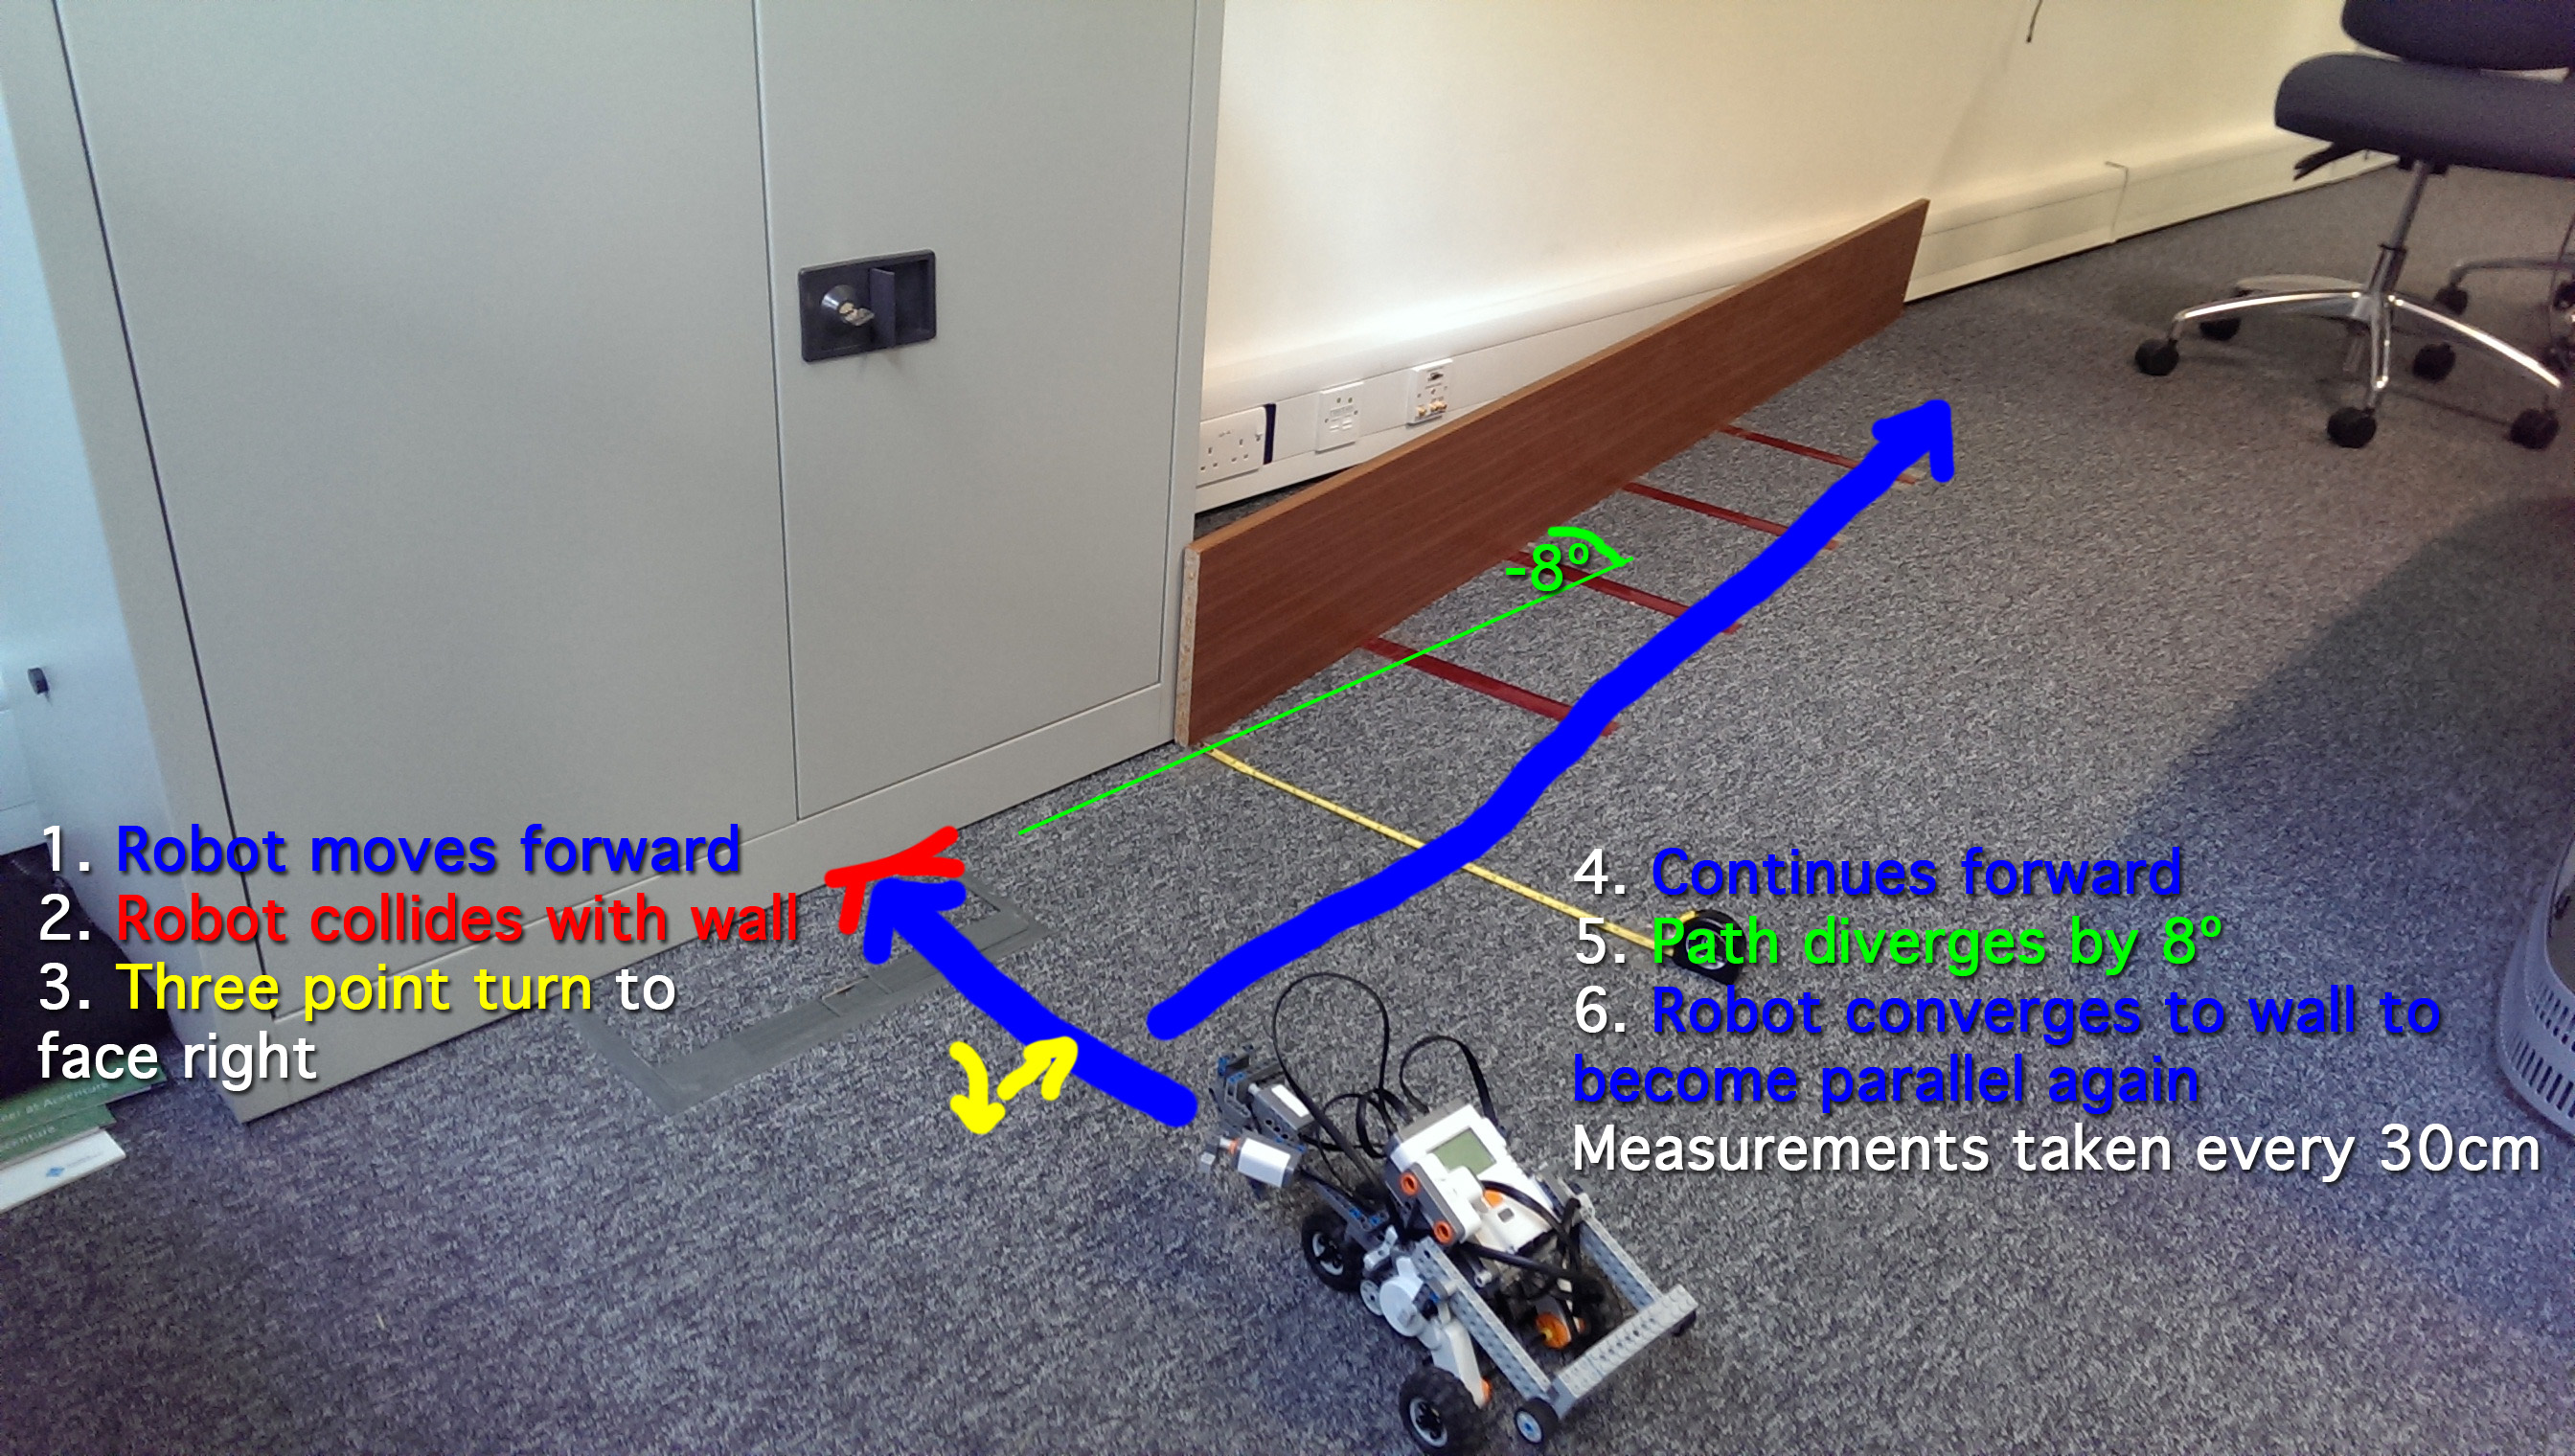
\includegraphics[width=8in]{CourseM8_Edit.jpg}}
\caption{\ang{-8} wall following (drawn path is an example for illustrative purposes)}
\label{fig:coursem8}
\end{figure}

\begin{figure}[ht]
\centerline{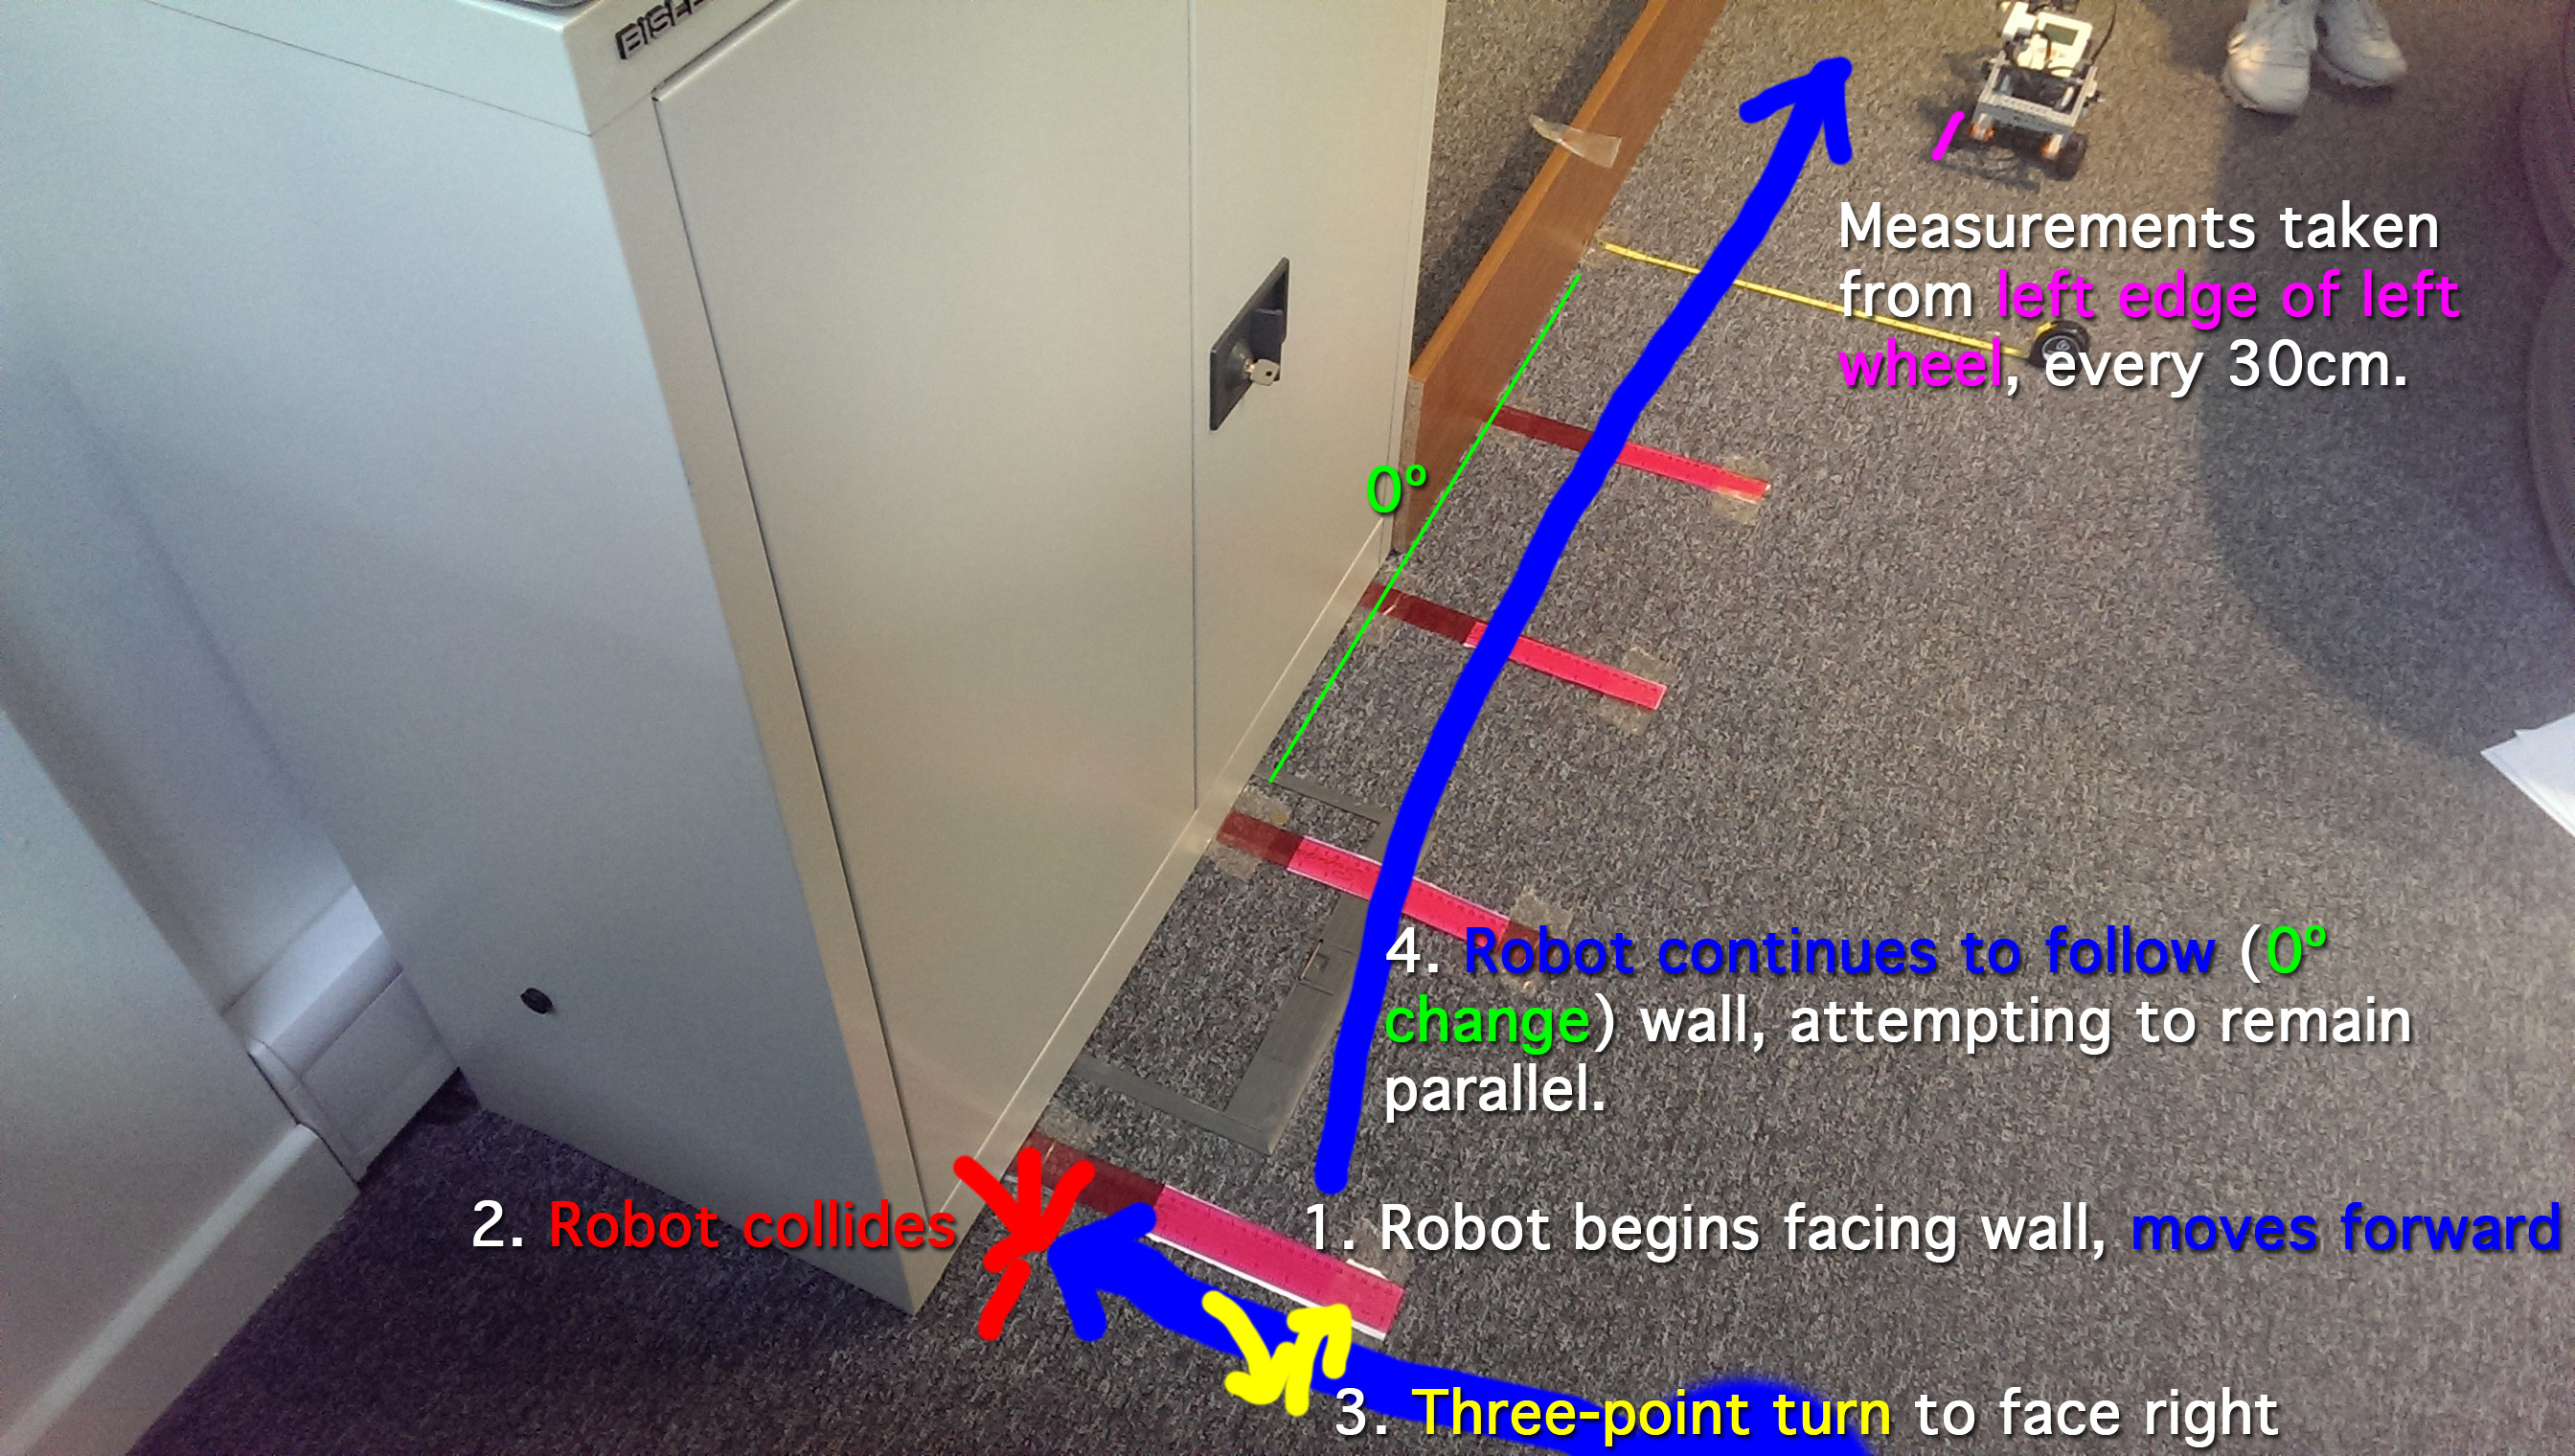
\includegraphics[width=8in]{Course0_Edit.jpg}}
\caption{\ang{0} wall following (drawn path is an example for illustrative purposes)}
\label{fig:course0}
\end{figure}

\begin{figure}[ht]
\centerline{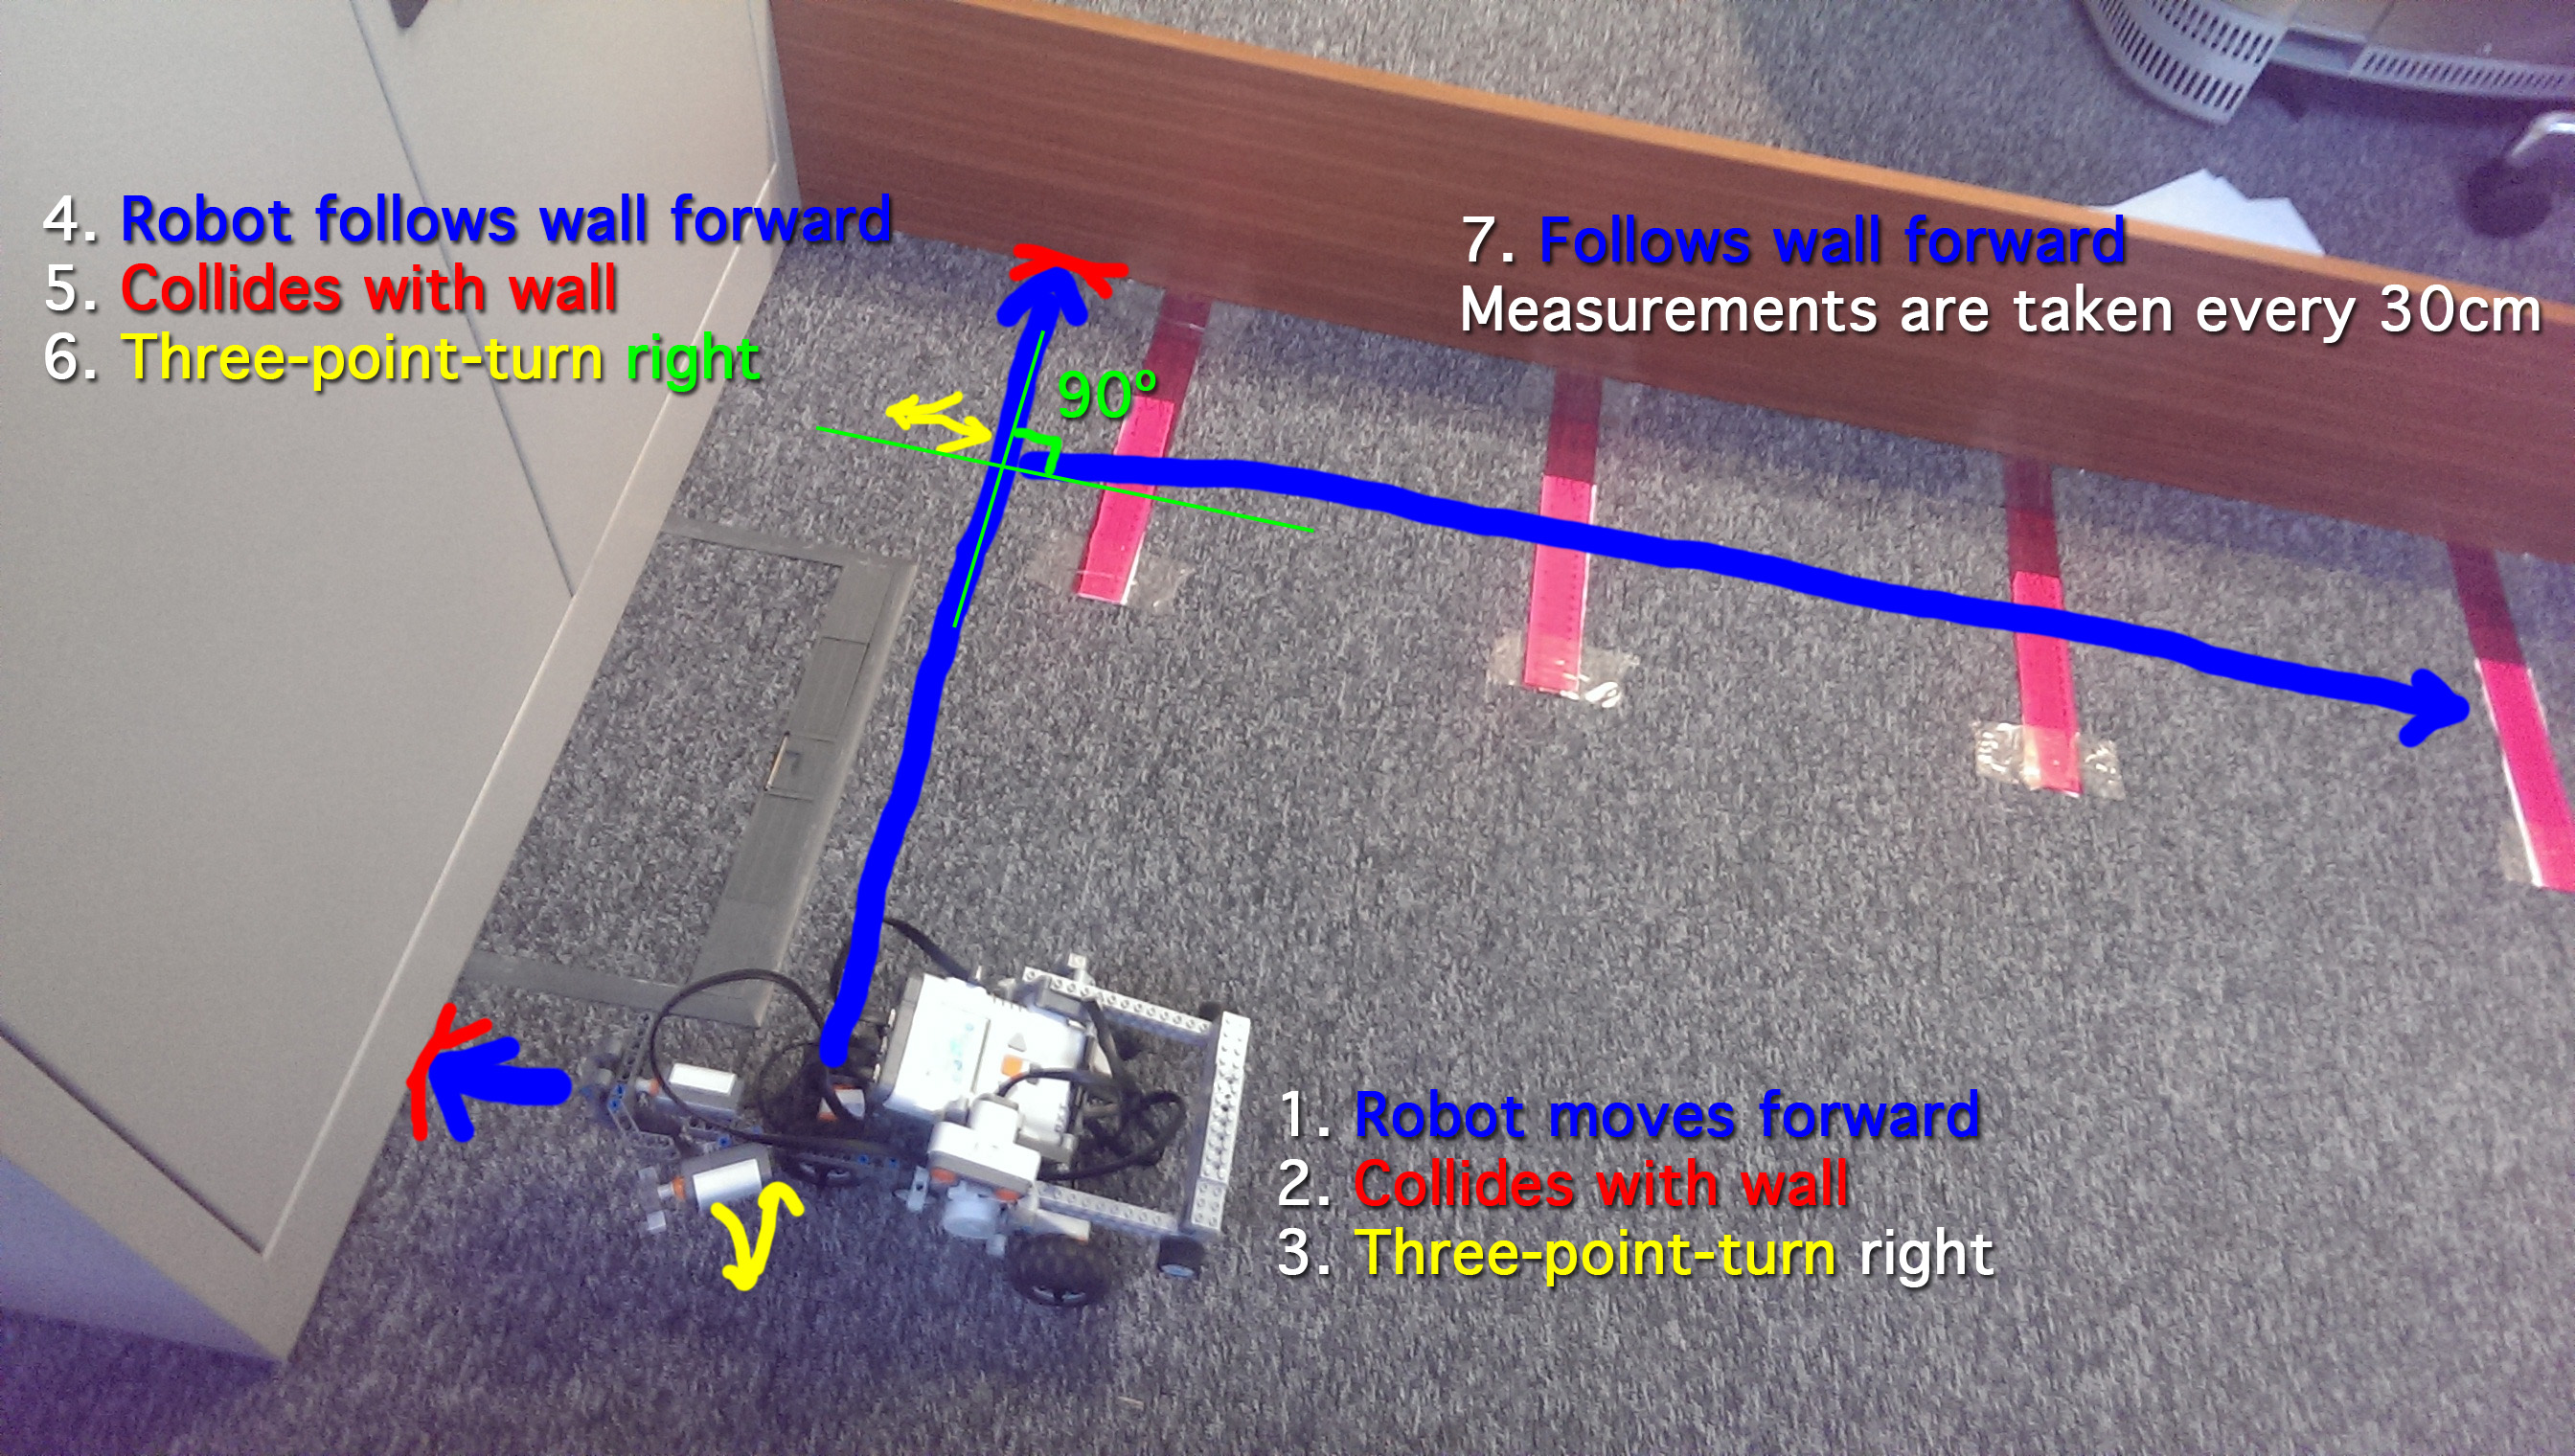
\includegraphics[width=8in]{Course90_Edit.jpg}}
\caption{\ang{90} wall following (drawn path is an example for illustrative purposes)}
\label{fig:course90}
\end{figure}


\begin{figure}[ht]
\begin{tabular}{c c c c c} % centered columns (4 columns) 
\hline\hline %inserts double horizontal lines 
Distance along wall (cm) & Attempt\#1 & Attempt\#2 & Attempt\#3 & Attempt\#4 \\ [0.5ex] % inserts table 
%heading 
\hline % inserts single horizontal line 
0 & 27 & 19 & 18 & 27\\
30 & 26 & 8 & 8 & 11\\
60 & 28 & 7 & 7 & 13\\
90 & 30 & 8 & 8 & 16\\
120 & 34 & 9 & 9 & 18\\ [1ex] % [1ex] adds vertical space 
\hline %inserts single line 
\end{tabular}
\caption{Raw data for wall separation at each milestone along wall after \ang{-90} turn}
\label{fig:rawm90}
\end{figure}

\begin{figure}[ht]
\begin{tabular}{c c c c c} % centered columns (4 columns) 
\hline\hline %inserts double horizontal lines 
Distance along wall (cm) & Attempt\#1 & Attempt\#2 & Attempt\#3 & Attempt\#4 \\ [0.5ex] % inserts table 
%heading 
\hline % inserts single horizontal line 
0 & 17 & 19 & 27 & 26\\
30 & 7 & 26 & 26 & 27\\
60 & 21 & 23 & 24 & 26\\
90 & 23 & 21 & 21 & 26\\
120 & 24 & 22 & 28 & 25\\ [1ex] % [1ex] adds vertical space 
\hline %inserts single line 
\end{tabular}
\caption{Raw data for wall separation at each milestone along wall after \ang{-8} turn}
\label{fig:rawm8}
\end{figure}

\begin{figure}[ht]
\begin{tabular}{c c c c c} % centered columns (4 columns) 
\hline\hline %inserts double horizontal lines 
Distance along wall (cm) & Attempt\#1 & Attempt\#2 & Attempt\#3 & Attempt\#4 \\ [0.5ex] % inserts table 
%heading 
\hline % inserts single horizontal line 
0 & 18 & 16 & 13 & 24\\
30 & 21 & 20 & 16 & 28\\
60 & 26 & 23 & 18 & 20\\
90 & 28 & 26 & 20 & 32\\
120 & 30 & 28 & 22 & 34\\ [1ex] % [1ex] adds vertical space 
\hline %inserts single line 
\end{tabular}
\caption{Raw data for wall separation at each milestone along wall after \ang{0} turn}
\label{fig:raw0}
\end{figure}

\begin{figure}[ht]
\begin{tabular}{c c c c c} % centered columns (4 columns) 
\hline\hline %inserts double horizontal lines 
Distance along wall (cm) & Attempt\#1 & Attempt\#2 & Attempt\#3 & Attempt\#4 \\ [0.5ex] % inserts table 
%heading 
\hline % inserts single horizontal line 
0 & 14 & 19 & 10 & 18\\
30 & 15 & 20 & 9 & 21\\
60 & 17 & 22 & 12 & 24\\
90 & 19 & 26 & 14 & 28\\
120 & 21 & 30 & 16 & 29\\ [1ex] % [1ex] adds vertical space 
\hline %inserts single line 
\end{tabular}
\caption{Raw data for wall separation at each milestone along wall after \ang{90} turn}
\label{fig:raw90}
\end{figure}



\begin{figure}[ht]
\begin{tabular}{c c c c c c c c} % centered columns (4 columns) 
\hline\hline %inserts double horizontal lines 
Dist travelled along wall (cm) & A\#1 & A\#2 & A\#3 & A\#4 & s.dev & mean & s.err \\ [0.5ex] % inserts table 
%heading 
\hline % inserts single horizontal line 
30 & 1 & 11 & 10 & 16 & 6.24 & 9.50 & 3.12\\
60 & 2 & 1 & 1 & 2 & 0.58 & 1.50 & 0.29\\
90 & 2 & 1 & 1 & 3 & 0.96 & 1.75 & 0.48\\
120 & 4 & 1 & 1 & 2 & 1.41 & 2.00 & 0.71\\ [1ex] % [1ex] adds vertical space 
\hline %inserts single line 
\end{tabular}
\caption{Delta in wall separation at each milestone along wall after \ang{-90} turn}
\label{fig:derivm90}
\end{figure}

\begin{figure}[ht]
\begin{tabular}{c c c c c c c c} % centered columns (4 columns) 
\hline\hline %inserts double horizontal lines 
Dist travelled along wall (cm) & A\#1 & A\#2 & A\#3 & A\#4 & s.dev & mean & s.err \\ [0.5ex] % inserts table 
%heading 
\hline % inserts single horizontal line 
30 & 10 & 7 & 1 & 1 & 4.50 & 4.75 & 2.25\\
60 & 14 & 3 & 2 & 1 & 6.06 & 5.00 & 3.03\\
90 & 2 & 2 & 3 & 0 & 1.26 & 1.75 & 0.63\\
120 & 1 & 1 & 7 & 1 & 3.00 & 2.50 & 1.50\\ [1ex] % [1ex] adds vertical space 
\hline %inserts single line 
\end{tabular}
\caption{Delta in for wall separation at each milestone along wall after \ang{-8} turn}
\label{fig:derivm8}
\end{figure}

\begin{figure}[ht]
\begin{tabular}{c c c c c c c c} % centered columns (4 columns) 
\hline\hline %inserts double horizontal lines 
Dist travelled along wall (cm) & A\#1 & A\#2 & A\#3 & A\#4 & s.dev & mean & s.err \\ [0.5ex] % inserts table 
%heading 
\hline % inserts single horizontal line 
30 & 3 & 4 & 3 & 4 & 0.58 & 3.50 & 0.29\\
60 & 5 & 3 & 2 & 8 & 2.65 & 4.50 & 1.32\\
90 & 2 & 3 & 2 & 12 & 4.86 & 4.75 & 2.43\\
120 & 2 & 2 & 2 & 2 & 0.00 & 2.00 & 0.00\\ [1ex] % [1ex] adds vertical space 
\hline %inserts single line 
\end{tabular}
\caption{Delta in wall separation at each milestone along wall after \ang{0} turn}
\label{fig:deriv0}
\end{figure}

\begin{figure}[ht]
\begin{tabular}{c c c c c c c c} % centered columns (4 columns) 
\hline\hline %inserts double horizontal lines 
Dist travelled along wall (cm) & A\#1 & A\#2 & A\#3 & A\#4 & s.dev & mean & s.err \\ [0.5ex] % inserts table 
%heading 
\hline % inserts single horizontal line 
30 & 1 & 1 & 1 & 3 & 1.00 & 1.50 & 0.50\\
60 & 2 & 2 & 3 & 3 & 0.58 & 2.50 & 0.29\\
90 & 2 & 4 & 2 & 4 & 1.15 & 3.00 & 0.58\\
120 & 2 & 4 & 2 & 1 & 1.26 & 2.25 & 0.63\\ [1ex] % [1ex] adds vertical space 
\hline %inserts single line 
\end{tabular}
\caption{Delta in wall separation at each milestone along wall after \ang{90} turn}
\label{fig:deriv90}
\end{figure}



\begin{figure}[ht]
\fbox{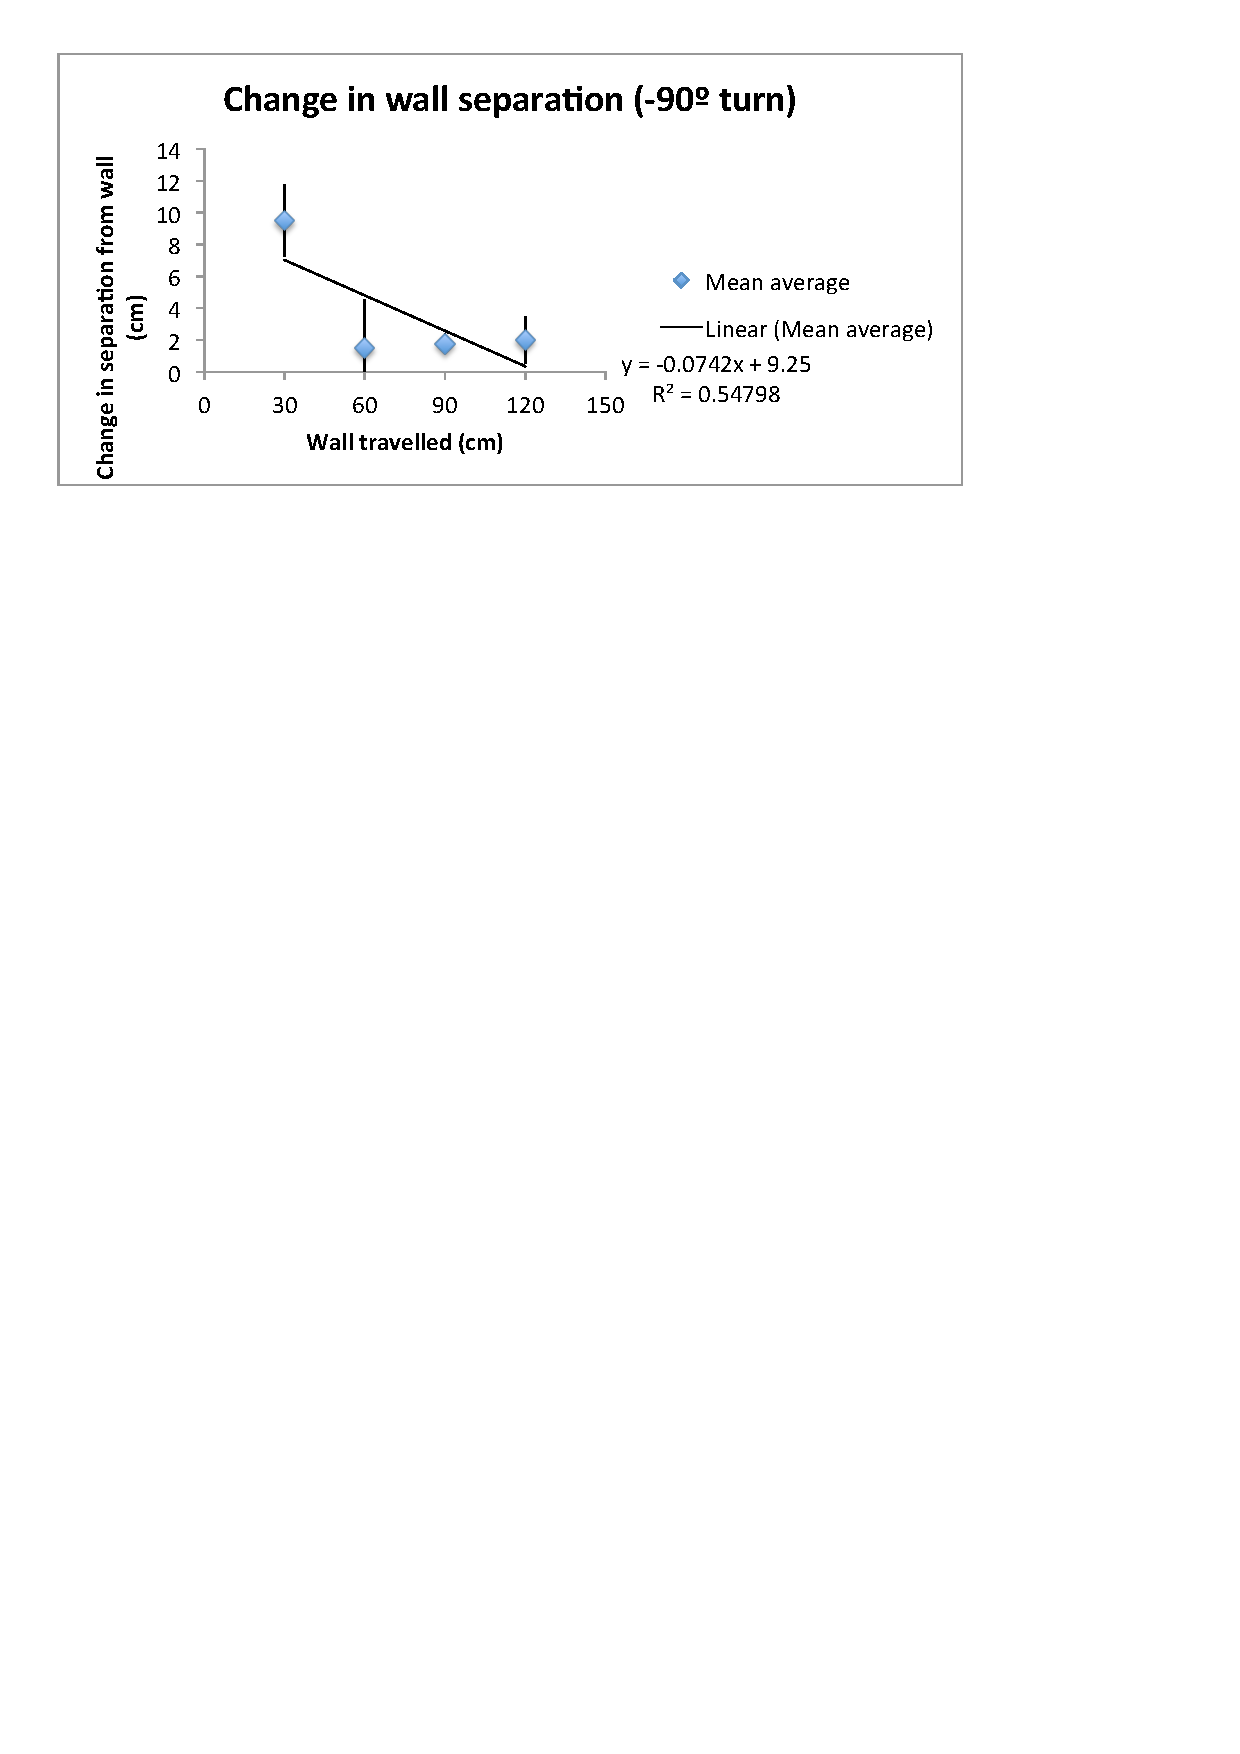
\includegraphics{TurnM90.pdf}}
\caption{Convergence to wall after a left-hand turn, over 4 attempts}
\label{fig:turnm90}
\end{figure}

\begin{figure}[ht]
\fbox{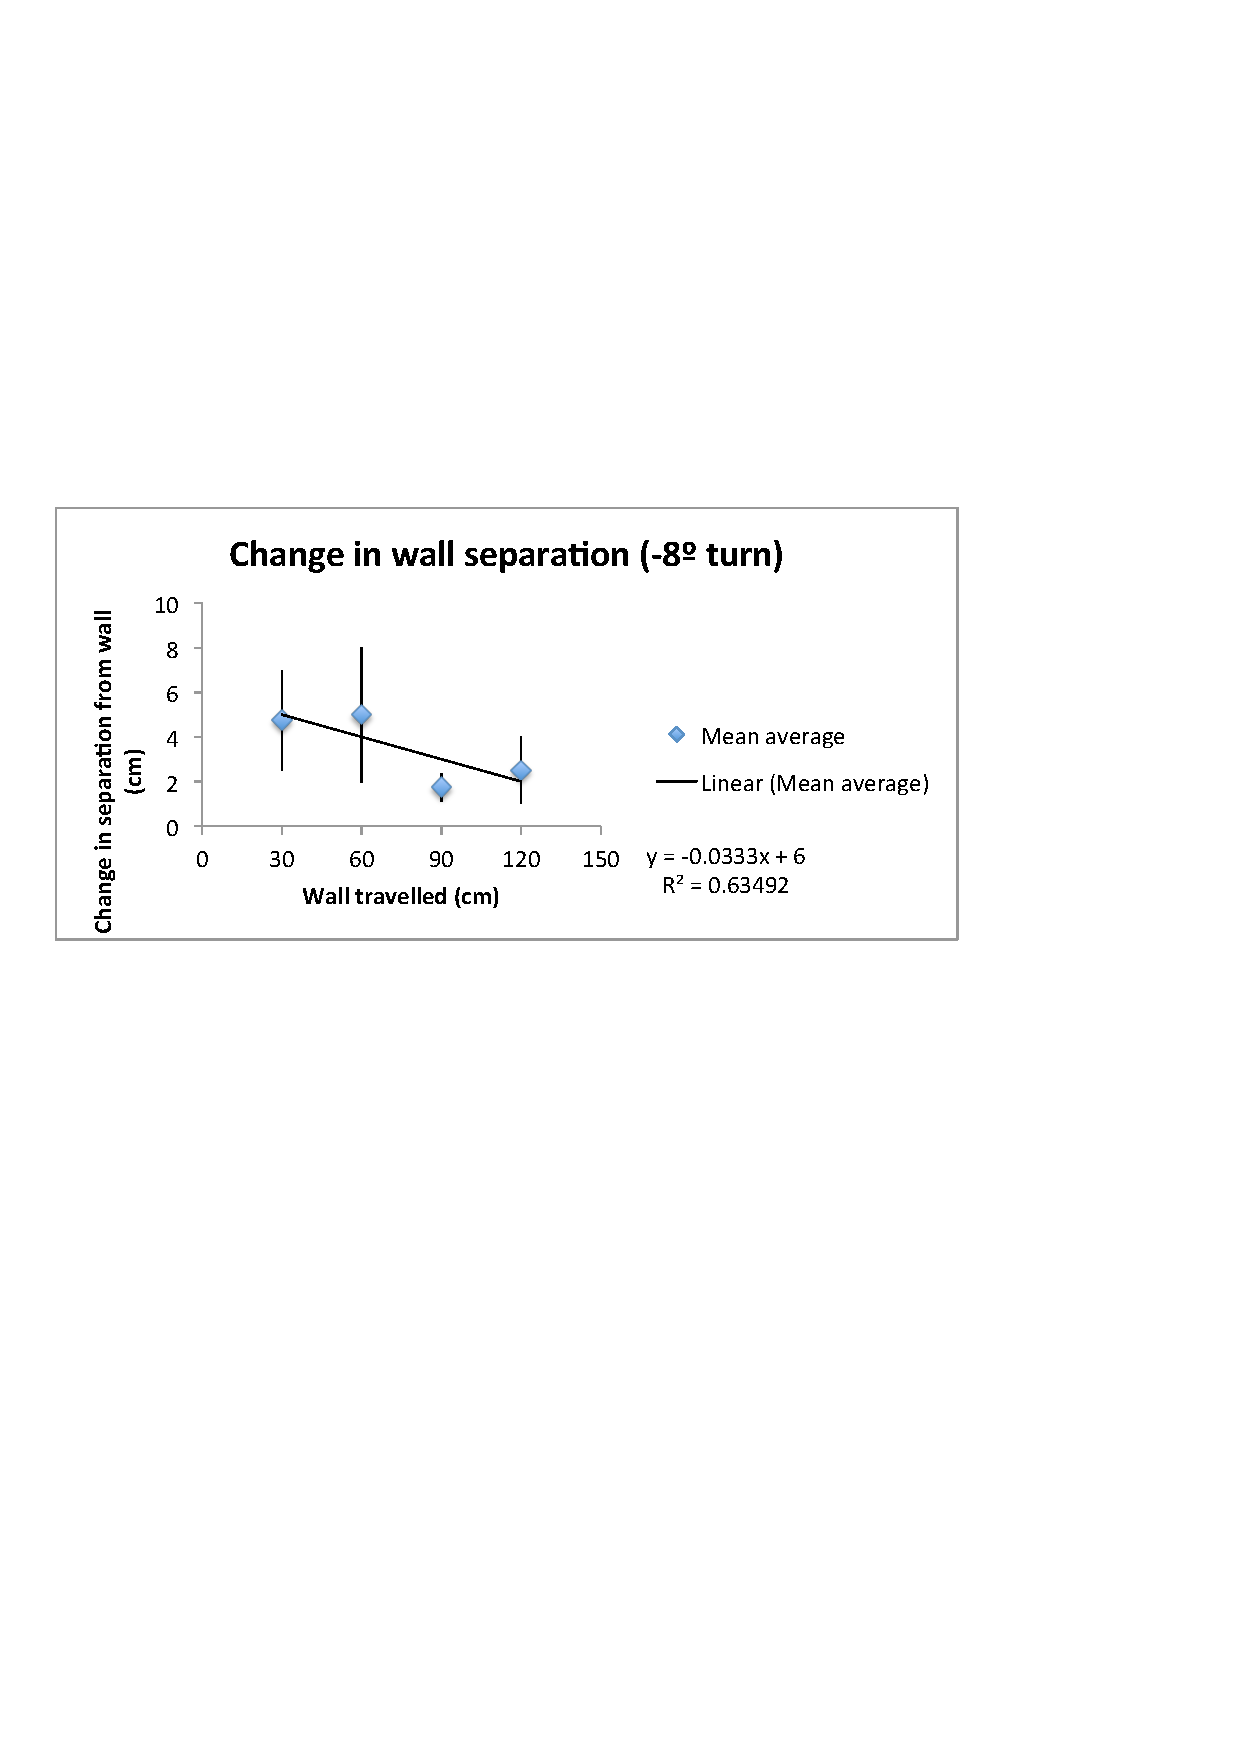
\includegraphics{TurnM8.pdf}}
\caption{Convergence to wall around slightly obtuse angle, over 4 attempts}
\label{fig:turnm8}
\end{figure}

\begin{figure}[ht]
\fbox{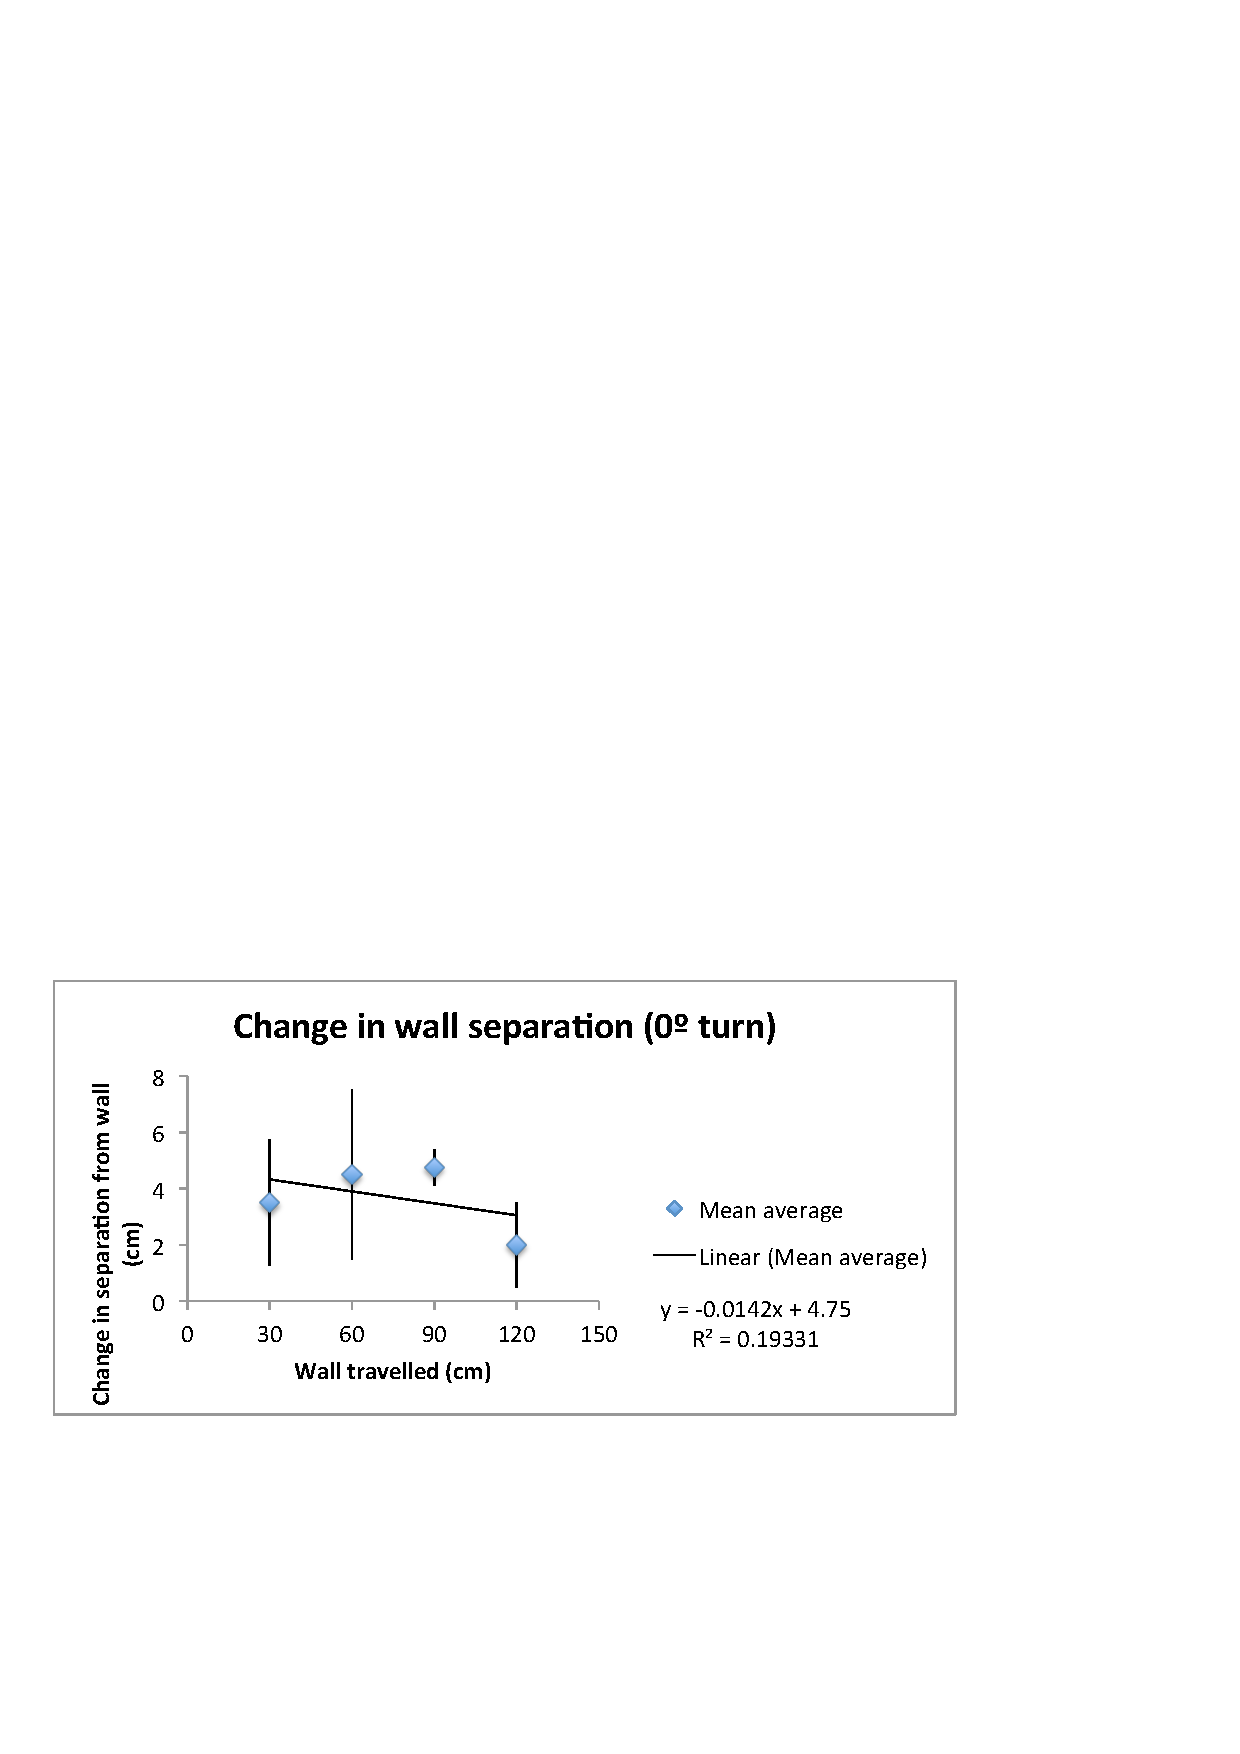
\includegraphics{Turn0.pdf}}
\caption{Continued convergence along a straight wall, over 4 attempts}
\label{fig:turn0}
\end{figure}

\begin{figure}[ht]
\fbox{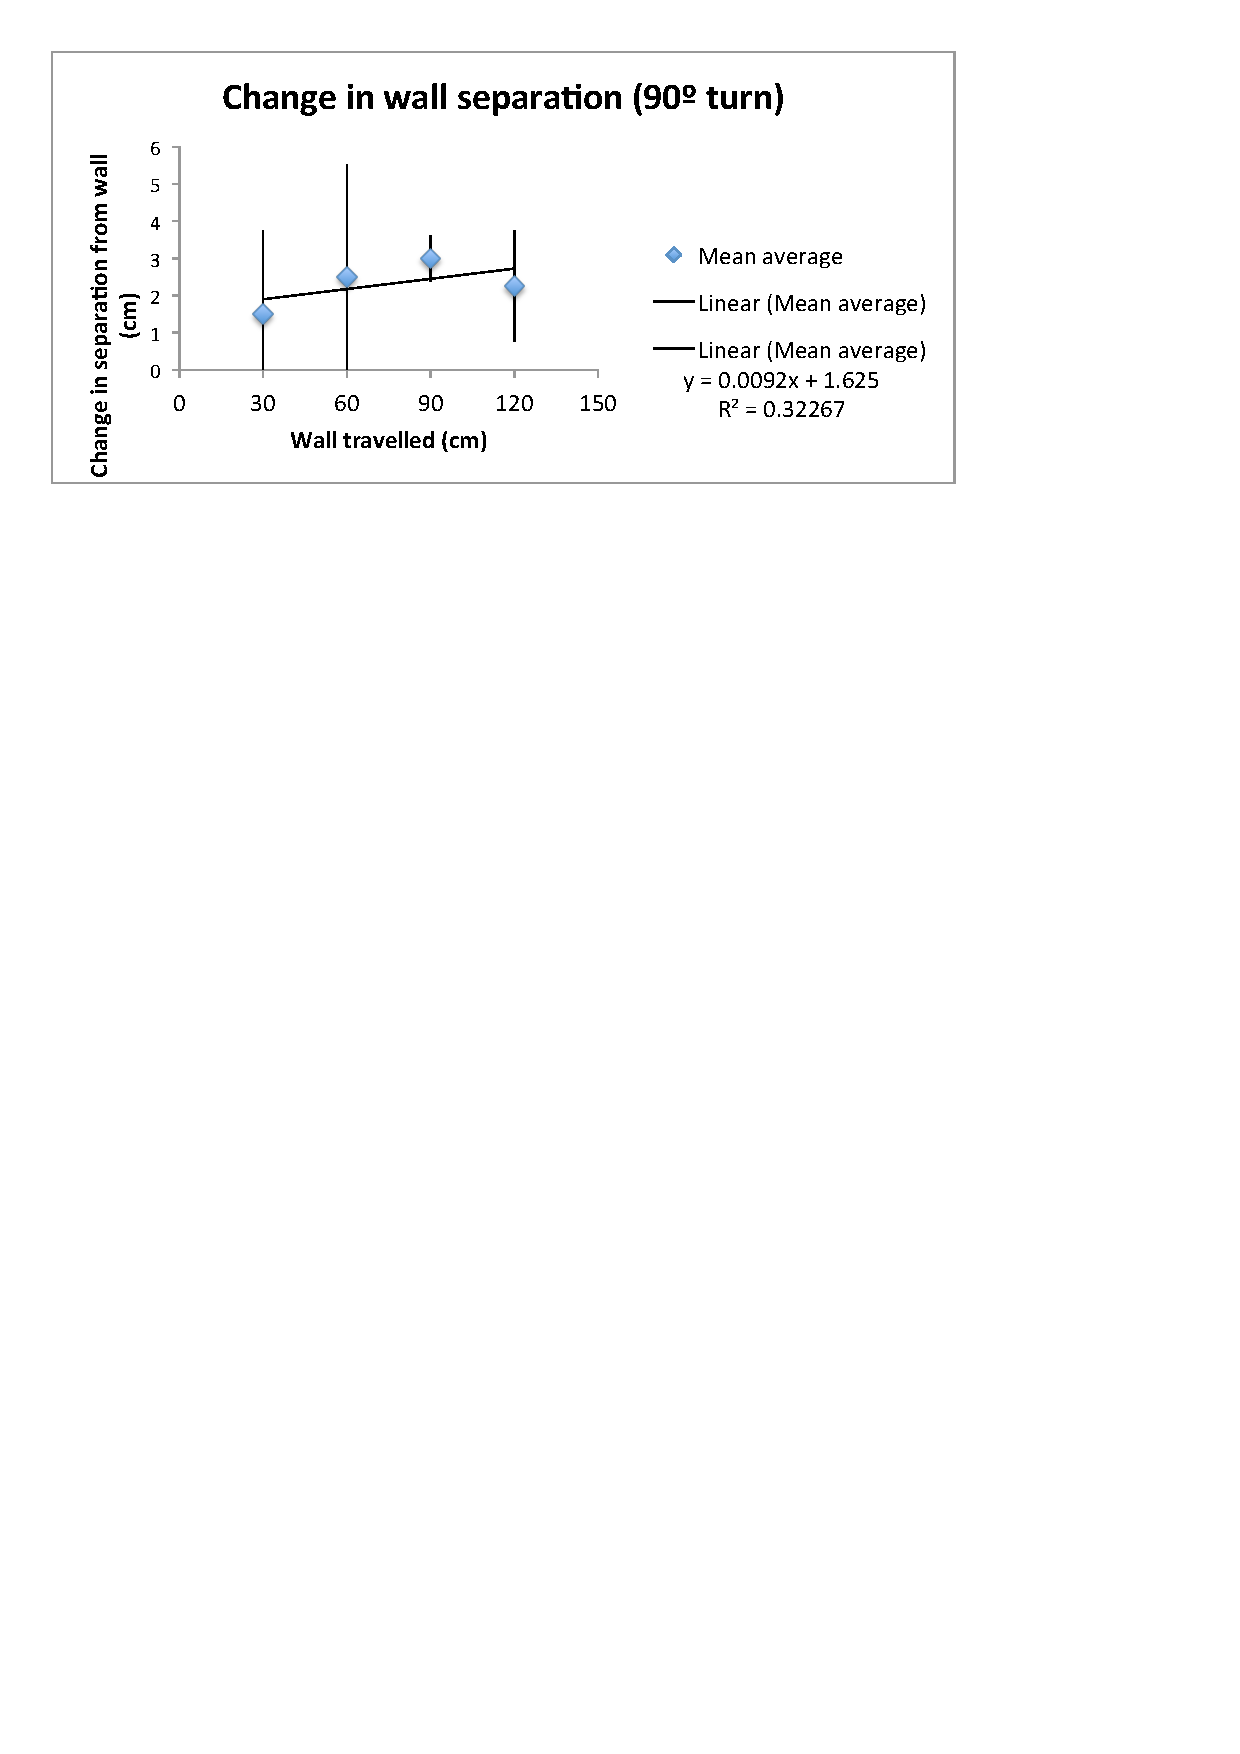
\includegraphics{Turn90.pdf}}
\caption{Convergence to wall after a right-hand turn, over 4 attempts}
\label{fig:turn90}
\end{figure}


\begin{figure}[ht]
\centerline{\includegraphics[width=8in]{TheRobot.jpg}}
\caption{The robot}
\label{fig:theRobot}
\end{figure}

\FloatBarrier

%\bibliographystyle{apalike}
%\bibliography{biblio}
\printbibliography

\end{document}
